\documentclass[9pt]{beamer}
\usefonttheme[onlymath]{serif}
\usepackage[sfdefault]{roboto}
\usepackage[utf8]{inputenc}
\usepackage[T1]{fontenc}
\usepackage{styles/fluxmacros} 	% Define where theme files are located. 
\usefolder{styles}
\usetheme[style=gray]{flux} % Available styles: asphalt, blue, red, green, gray 



\usepackage{graphicx}
\usepackage{amsmath}
\usepackage{amssymb}
\usepackage{amsfonts}
\usepackage{hyperref}

\title{Computerpraktikum Maschinelles Lernen}
\subtitle{Thema 4 - Klassifikationsverfahren}
\author{Pascal Bauer, Raphael Millon, Florian Haas}
\institute{Sommersemester 2020}
\date{\today}
\titlegraphic{assets/Empty.png}

\begin{document}

\titlepage 

\begin{frame}
 \frametitle{Table of contents}
 \tableofcontents
\end{frame}

\section{Theorie}
\begin{frame}{Theorie}{Theorie}

\end{frame}

\section{Showcase}
\begin{frame}{Showcase}{Showcase}

\end{frame}

\section{Ausgesuchte Codebeispiele}
\begin{frame}{Codebeispiele}{Struktur und Module}
Code ist Open-Source auf Github: \url{https://github.com/raphaelMi/computerpraktikum-maschinelles-lernen}\\[0.4em]
Unser Programm ist in folgende Module aufgeteilt:
\begin{itemize}
\item{\textbf{main.py}: Hauptmodul mit wesentlichen Algorithmen}
\item{\textbf{dataset.py}: Datensatz-Import/-Export}
\item{\textbf{gui.py}: Grafische Oberfläche}
\item{\textbf{kd\_tree.py}: Hilfsmodul für k-d-Search}
\item{\textbf{visual.py}: Plotting der Datensätze}
\end{itemize}

Verwendete Bibliotheken:
\begin{itemize}
\item{\textbf{numpy}: Effizientes (vektorisiertes) Rechnen}
\item{\textbf{matplotlib}: Generieren der Plots}
\item{\textbf{tkinter}: Grafische Benutzeroberflächen}
\item{\textbf{scikit-learn}: Ein dritter Algorithmus zum Vergleich}
\end{itemize}
\end{frame}
\begin{frame}{Codebeispiele}{Klassifikation}
Die \textbf{classify}-Funktion ist das "Herz" unseres Programmes:
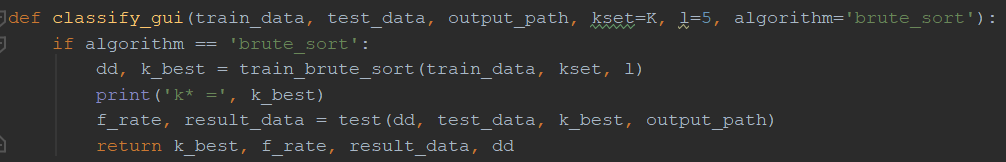
\includegraphics[scale=0.633]{assets/classify_brute.png}\\[0.4em]
Parameter:
\begin{itemize}
\item{\textbf{train\_data}: Trainingsdaten}
\item{\textbf{train\_data}: Testdaten}
\item{\textbf{output\_path}: Ausgabedatei der Ergebnisdaten}
\item{\textbf{kset}: Menge der k}
\item{\textbf{l}: Partitionsanzahl}
\item{\textbf{algorithm}: Suchalgorithmus für Nachbarn}
\end{itemize}
Ablauf:
\begin{enumerate}[1.]
\item{Training mit gegebenen Trainingsdaten und Sortieralgorithmus}
\item{Klassifikation und der Testdaten und Darstellung der Resultate}
\end{enumerate}
\end{frame}
\end{document}